%
% Thesis Style 用サンプル TeX
%
% 注意:目次等を作成するために何度か platex にかけること
%
% 両面印刷する時は twoside にする
%
\documentclass[12pt,twoside]{jsbook}
\usepackage{csg-thesis}

\usepackage[dvipdfmx]{graphicx}
\usepackage{url}
\usepackage{amsmath,amssymb}

\begin{document}

% 題目
% 適当に\\で区切って見やすくする
\title{ {{ .Title }} }

% 学位(学部と大学院で変更)
{{- if eq .Degree "bachelor" }}
\degree{学士}
{{- else }}
\degree{修士}
{{- end }}

% 名前
\author{ {{ .Author.Name }} }

% 提出日
\date{ {{ .Year }} 年1月}

% 卒業年度
\schoolyear{ {{ .Year }}年}

% 所属(学部と大学院で変更)
\department{ {{ .Author.Affiliation.University }} {{ .Author.Affiliation.Department }}}

% 学籍番号
\stnumber{ {{ .Author.StudentId }}}

% 指導教員(教官ではなくなった...)
\supervisor{ {{ .Supervisors }}}

\maketitle

%%%%%%%%%%%%%%%%%%%%%%%%%%%%%%%%%%%%%%%%%%%%%%%%%%%%%%%%%%%%%%%%%%%%%%

% 概要
\begin{abstract}
    論文の概要を書こう.概要は,論文の内容を簡潔に400字〜600字程度でまとめたものである.
    なぜその研究が必要なのか,どのようなアプローチで取り組んだのか,そして,どのような結果が得られたのかなどを書く.
    この概要を読むことで,論文の全体像が掴めるようになるのが理想である.

    この文書は,\LaTeX の使い方の説明や例を示すためのサンプルであるとともに,卒業論文の書き方の説明を兼ねている.
    この文書のソースコードを確認しながら,自分の卒論の文章に置き換えていってもらいたい.
\end{abstract}

% 謝辞
\begin{acknowledgments}
誰にどのようにお世話になったのかを書く.
多くの場合,所属研究室の先輩や教員,友人などに感謝の意を述べる.
また,研究を進める上での助言や協力をしてくれた人にも感謝の意を述べる.
感謝を述べるときには,してもらったことを具体的に書くと良い.
\end{acknowledgments}

%%%%%%%%%%%%%%%%%%%%%%%%%%%%%%%%%%%%%%%%%%%%%%%%%%%%%%%%%%%%%%%%%%%%%%

\pagenumbering{roman}  %% ページ番号をローマ数字にする
\tableofcontents       %% 目次

%
% 目次等にはローマ数字を使い、本文開始ページを 1 ページ目にできる
% この方が見た目がきれいであるが、全体のページ数は減って見える
% ここでローマ数字に変えた場合は chapter 1 でアラビア数字に戻すこと
%

\listoffigures         %% 図目次(図がない場合は不要)
\listoftables          %% 表目次(表がない場合は不要)

\ownpaper              %% 関連発表文献リスト(必要ならコメントを外す)

\begin{enumerate}
\item hogehoge
\end{enumerate}

%%%%%%%%%%%%%%%%%%%%%%%%%%%%%%%%%%%%%%%%%%%%%%%%%%%%%%%%%%%%%%%%%%%%%%

\pagenumbering{arabic}  %% ページ番号をアラビア数字に変更

%
% 本文
%
\chapter{はじめに}

\section{\LaTeX の心得}

\LaTeX はマークアップ言語である.
そのため,基本的に文章を書けばその通りに出力される.
そして,自分自身で細かいレイアウトの調整をしようとしないことが大切である.
ページのどこに何を置きたいかは考えずに,文章の中身に集中しよう.

\LaTeX を書くうえで,最低限知っておくべきルールは次の通りである.

\begin{itemize}
    \item 改行,半角スペースは無視される.
    \item 空行を入れる(2回以上の改行)と段落が変わる.
\end{itemize}

Webで検索すると色々と情報が出てくるが,\LaTeX は古いソフトウェアであるため,情報が古いものが多い.
そのため基本的には\textbf{TeX Wiki}\footnote{\url{https://texwiki.texjp.org/}}を参照すると良い.


\section{\LaTeX のインストール}

macOSに \LaTeX をインストールするには,Homebrew を使おう\footnote{\url{https://texwiki.texjp.org/?MacTeX}}.
非常に大容量のパッケージであるため,常時接続環境でインストールに臨もう.

\begin{verbatim}
    $ brew install --cask mactex
    $ sudo tlmgr update --self --all
    $ sudo tlmgr paper a4
\end{verbatim}

\section{\LaTeX での画像貼り付け}

画像はベクタ形式のPDFを使う.eps形式は前世紀の遺物であるため今の時代は使わない.
間違ってもラスタ形式は使わないこと.
特にグラフをラスタ形式にすることは厳禁である.

以下のようなコードを書くと,画像が貼り付けられる.
ここで,\verb!\centering! は画像を中央に配置するためのコマンドであり,
\verb!\includegraphics!で実際に画像を貼り付ける.
\verb![width=3cm]! は画像の幅を指定している.他にも,{\texttt height}などでも指定できる.
画像の拡張子は省略する.
\verb!caption!は画像のキャプション(説明)であり,省略は不可である.
\verb!label!は画像を参照するためのラベルである.
画像を参照する場合「図\verb!\ref{fig:image_label}!」のように書くと「図1.1」のように参照できるようになる.

\begin{verbatim}
\begin{figure}[b]
    \centering
    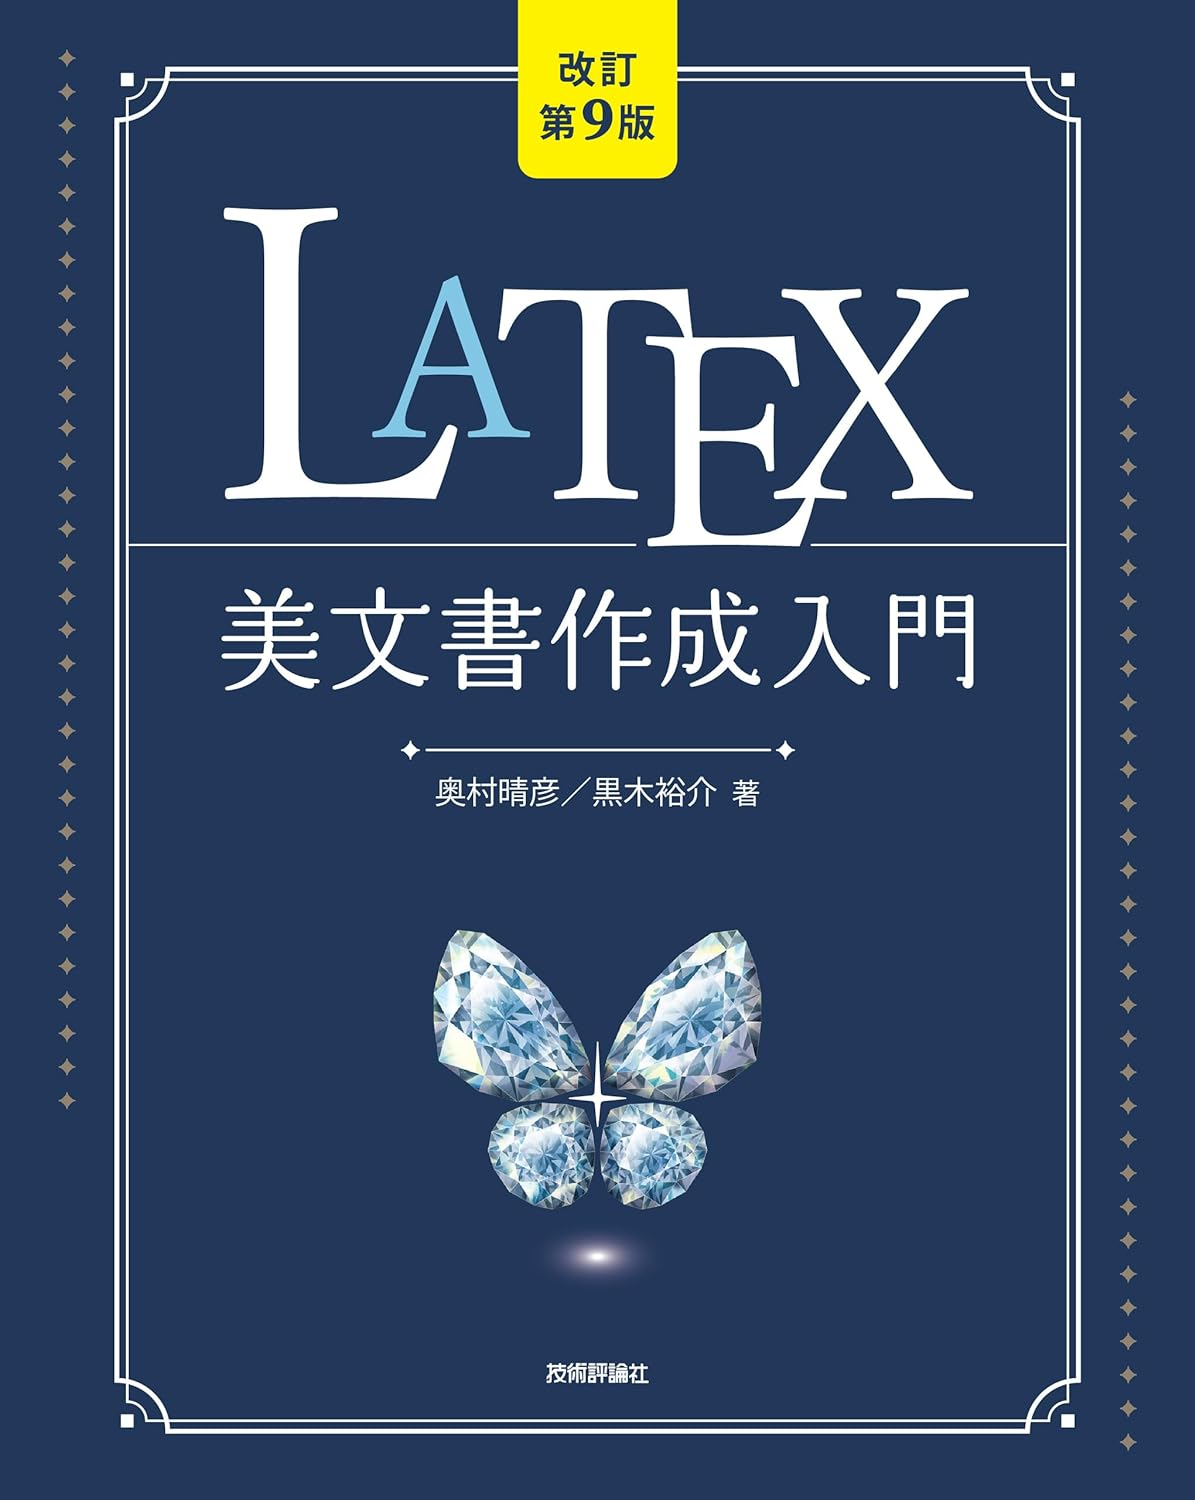
\includegraphics[width=3cm]{images/4297138891}
    \caption{画像の説明(省略は不可)}
    \label{fig:image_label}
\end{figure}
\end{verbatim}

複数の画像をまとめて表示したい場合は,\verb!minipage!環境と\verb!subcaption!パッケージを使う.
\verb!subfigure!や\verb!subfig!パッケージは遺物であるため,使わない.
具体的な方法はググろう.



\section{\LaTeX の参考資料}

\LaTeX を詳しく知りたい人は,図\ref{fig:okumura_latex}, \ref{fig:mizutani_latex}に挙げている書籍を読もう.

\begin{figure}[b]
    \begin{minipage}[t]{0.48\textwidth}
        \centering
        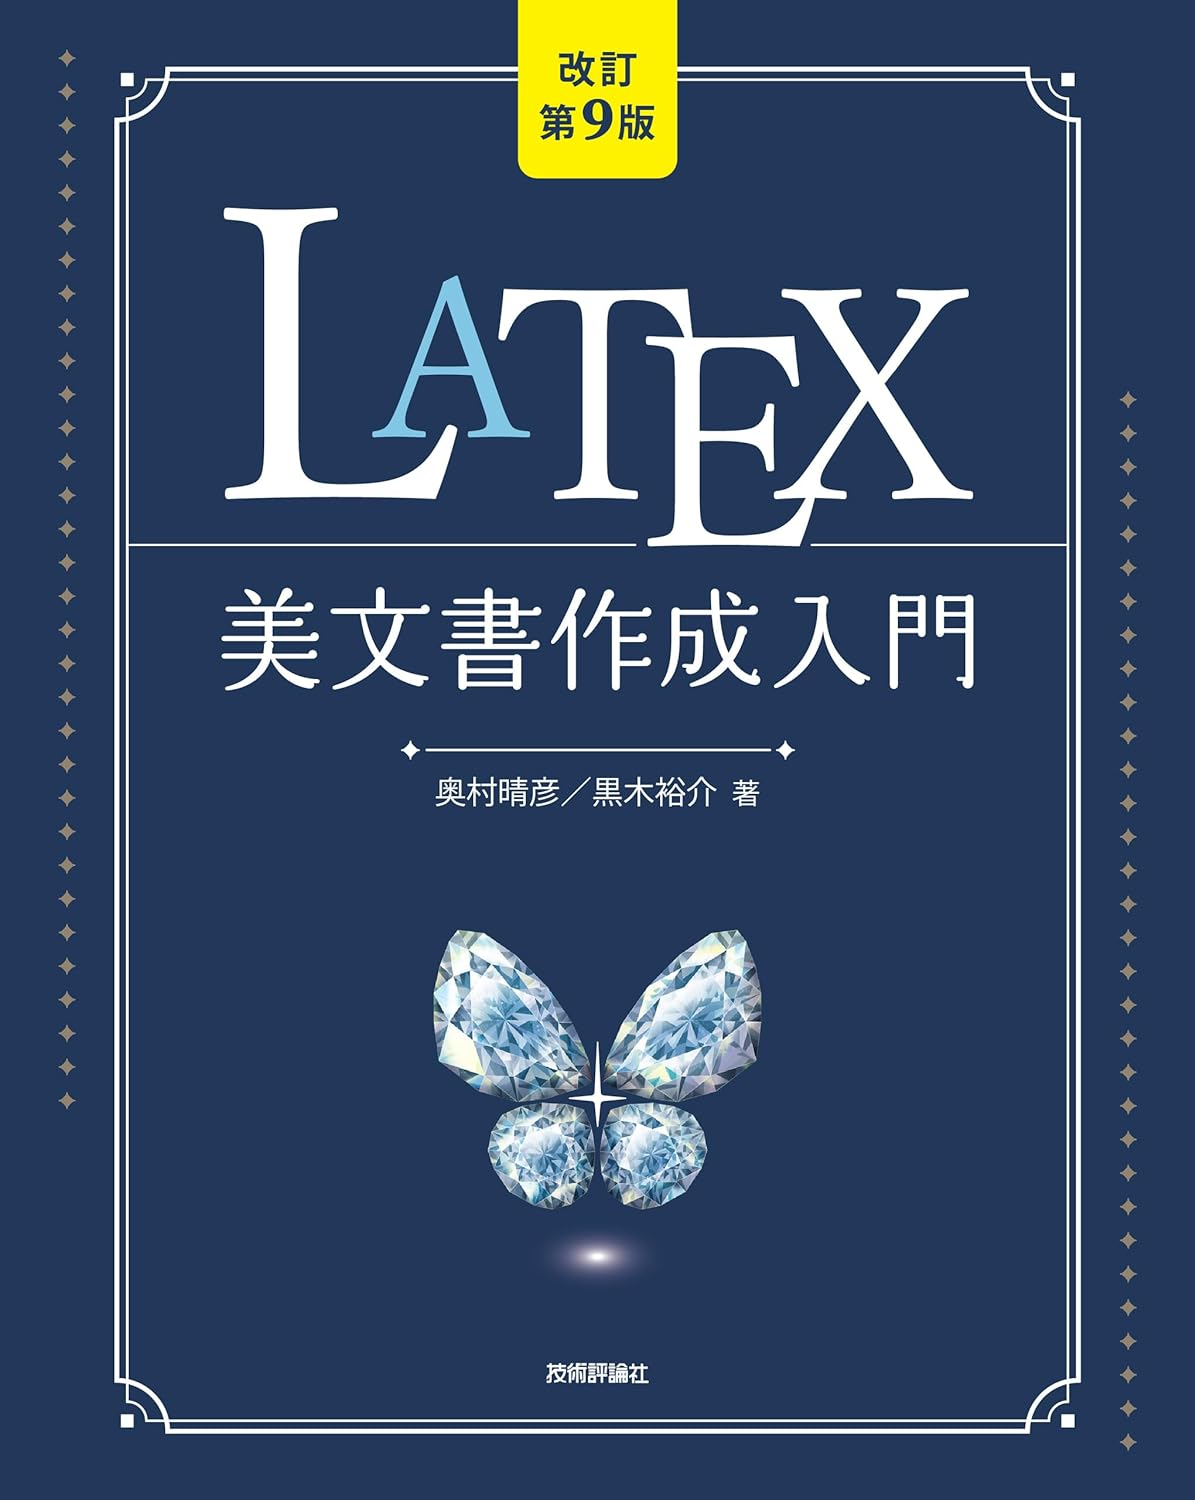
\includegraphics[height=5cm]{images/4297138891}
        \caption{[改訂第9版]\LaTeX 美文書作成入門\cite{2023okumura_book}}
        \label{fig:okumura_latex}
    \end{minipage}
    \begin{minipage}[t]{0.48\textwidth}
        \centering
        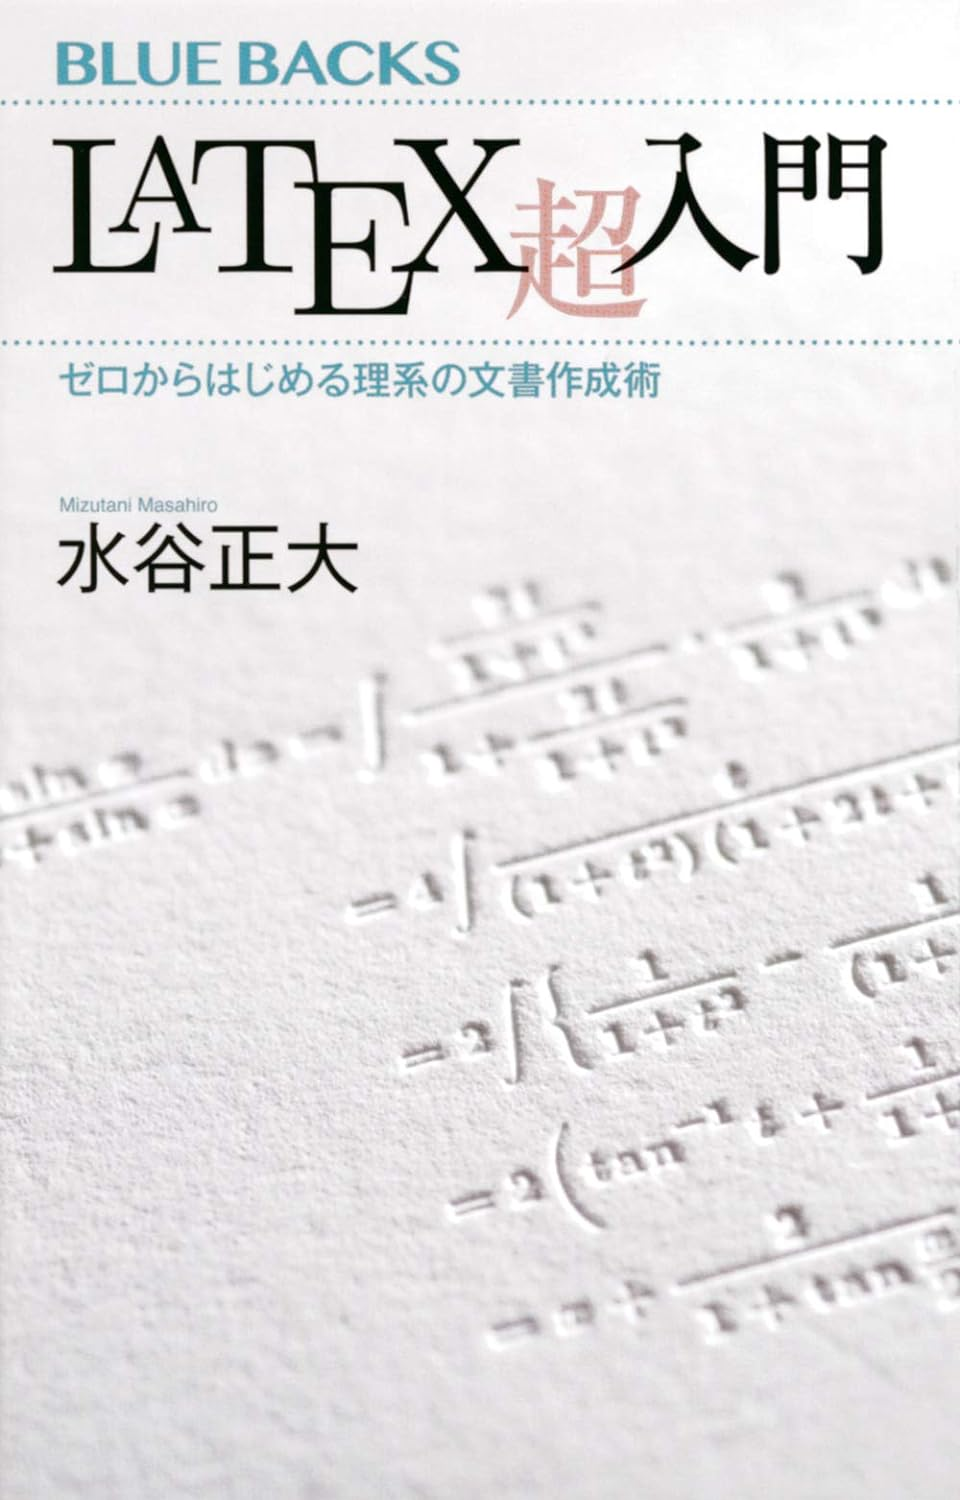
\includegraphics[height=5cm]{images/4065204968}
        \caption{\LaTeX 超入門 ゼロからはじめる理系の文書作成術\cite{2020mizutani_book}}
        \label{fig:mizutani_latex}
    \end{minipage}
\end{figure}

\section{作文の心得}

構造化された文章を書くことを意識しよう.
構造化された文章とは,章,節,小節,段落,文というように,階層的に書かれた文章のことである.
そのような文章を書くために,図\ref{fig:kinoshita_book}〜\ref{fig:tak_book}に挙げた4つの本のうち,どれか一つは読もう.

\begin{figure}[b]
    \begin{minipage}[t]{0.245\textwidth}
        \centering
        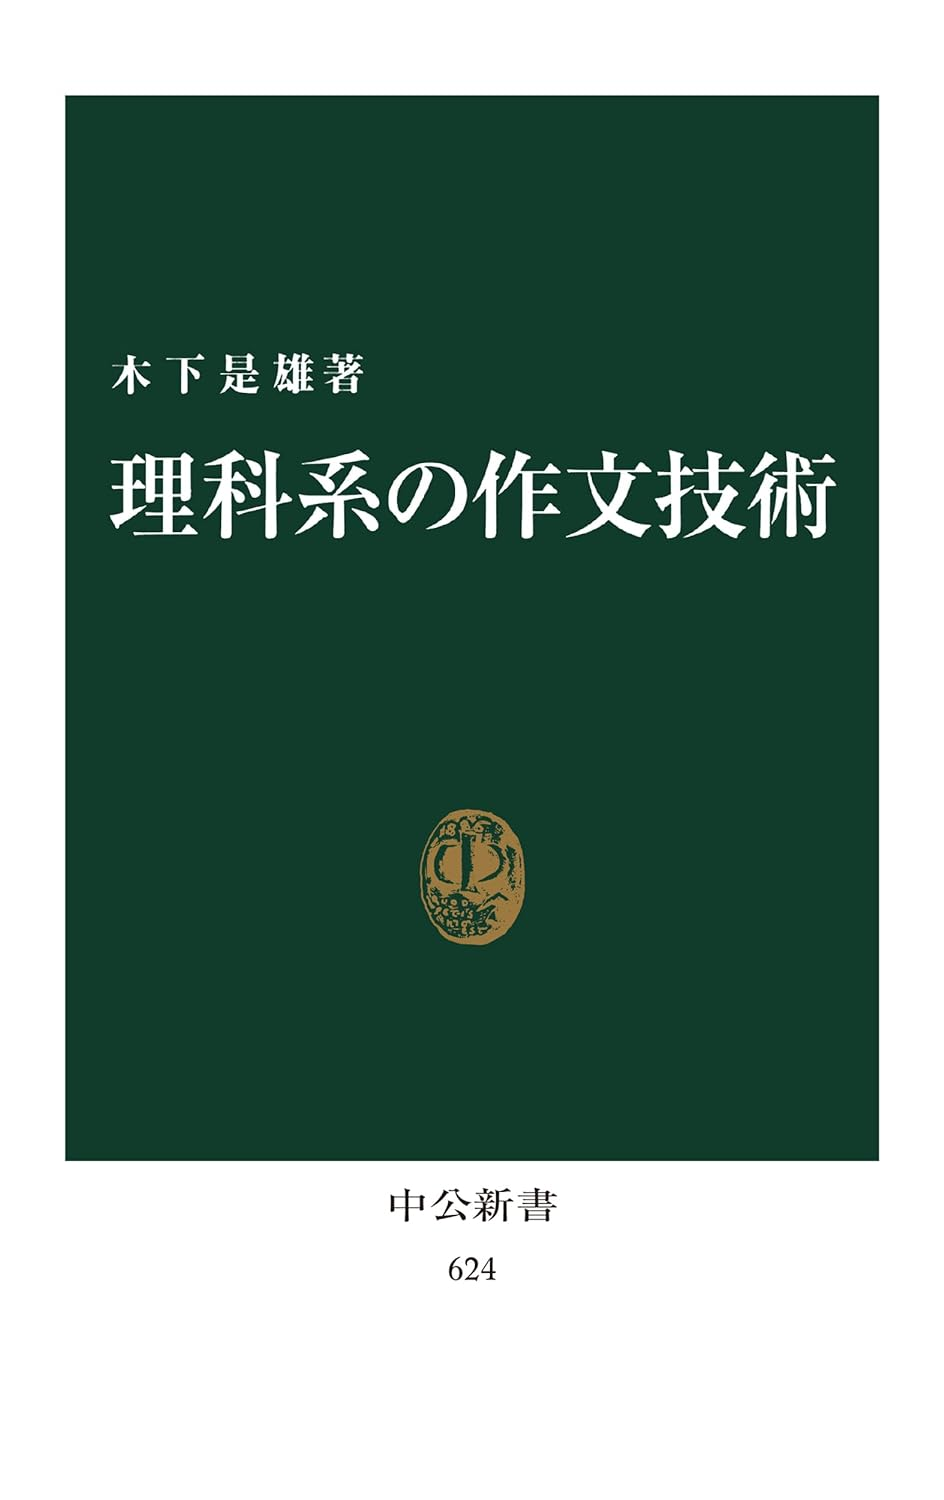
\includegraphics[height=3cm]{images/4121006240}
        \caption{理科系の作文技術\cite{1981kinoshita_book}}
        \label{fig:kinoshita_book}
    \end{minipage}
    \begin{minipage}[t]{0.245\textwidth}
        \centering
        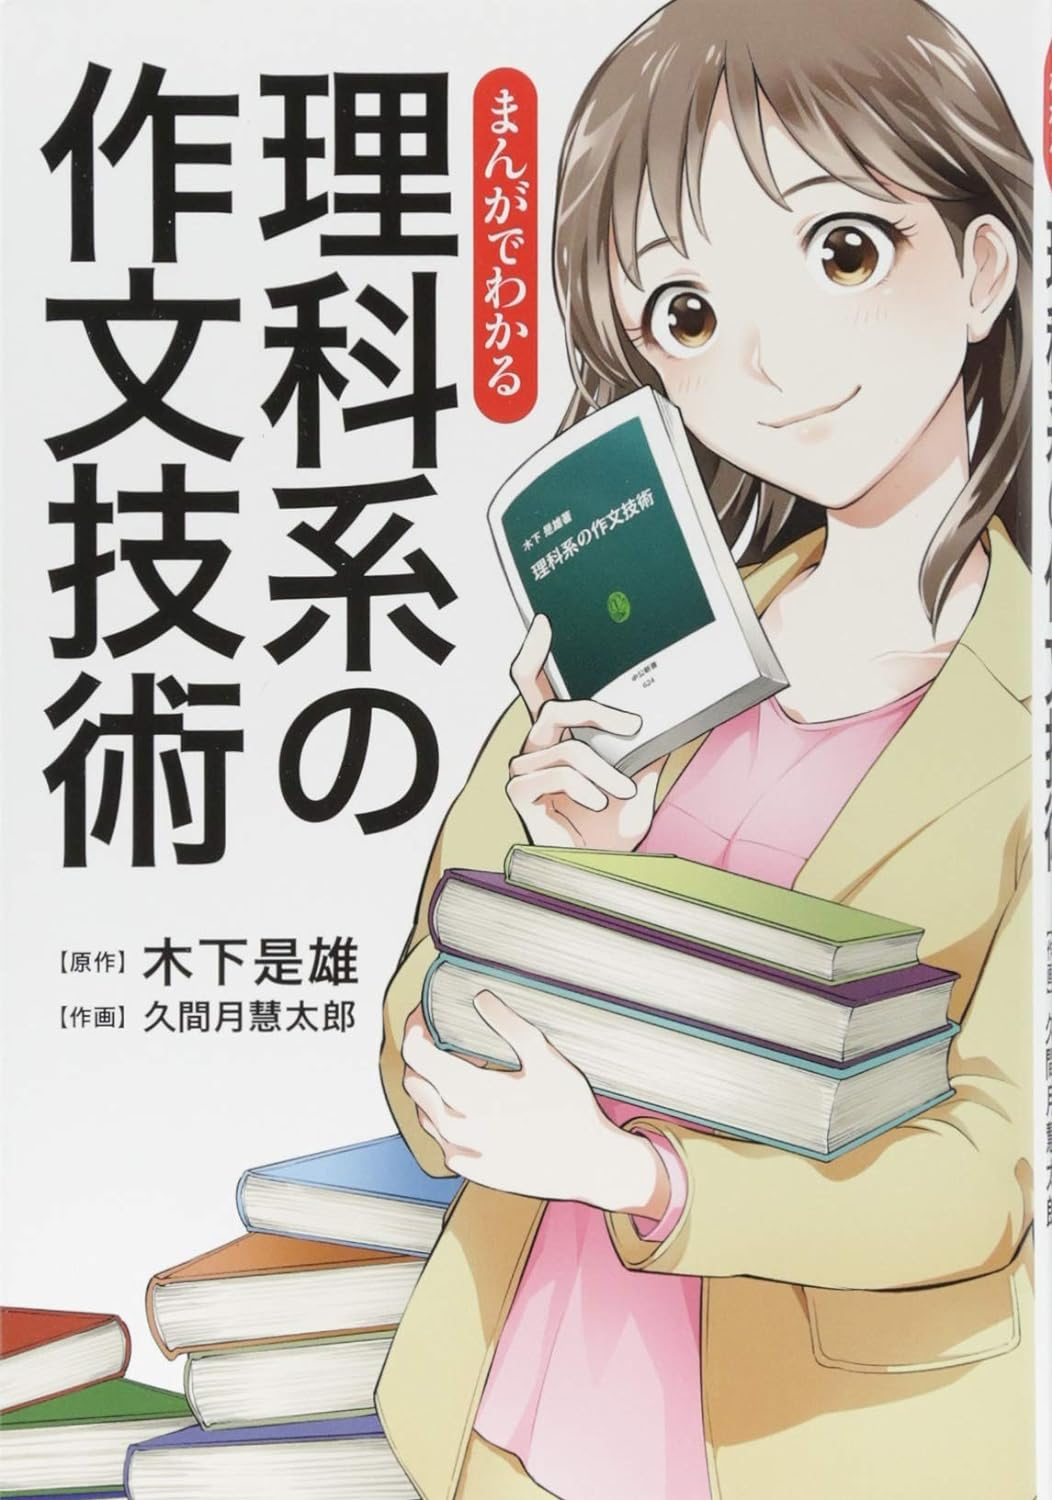
\includegraphics[height=3cm]{images/4120050424}
        \caption{まんがでわかる 理科系の作文技術 \cite{2018kumazuki_book}}
        \label{fig:kumazuki_book}
    \end{minipage}
    \begin{minipage}[t]{0.245\textwidth}
        \centering
        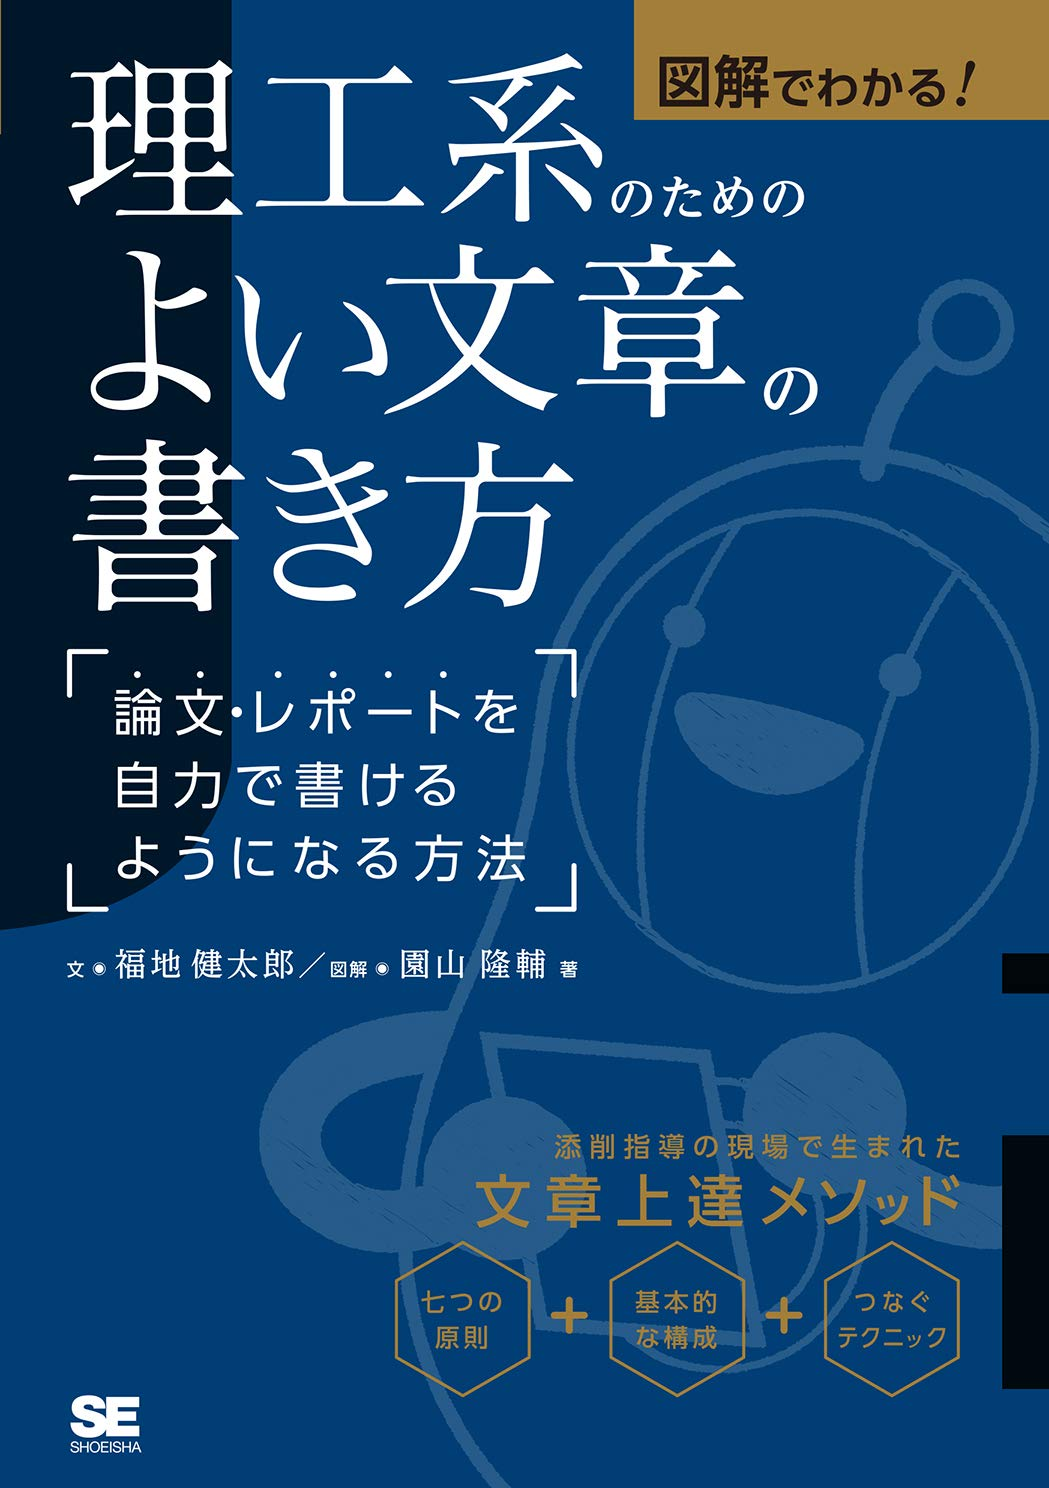
\includegraphics[height=3cm]{images/4798158895}
        \caption{図解でわかる! 理工系のためのよい文章の書き方 論文・レポートを自力で書けるようになる方法\cite{2019fukuchi_book}}
        \label{fig:fukuchi_book}
    \end{minipage}
    \begin{minipage}[t]{0.245\textwidth}
        \centering
        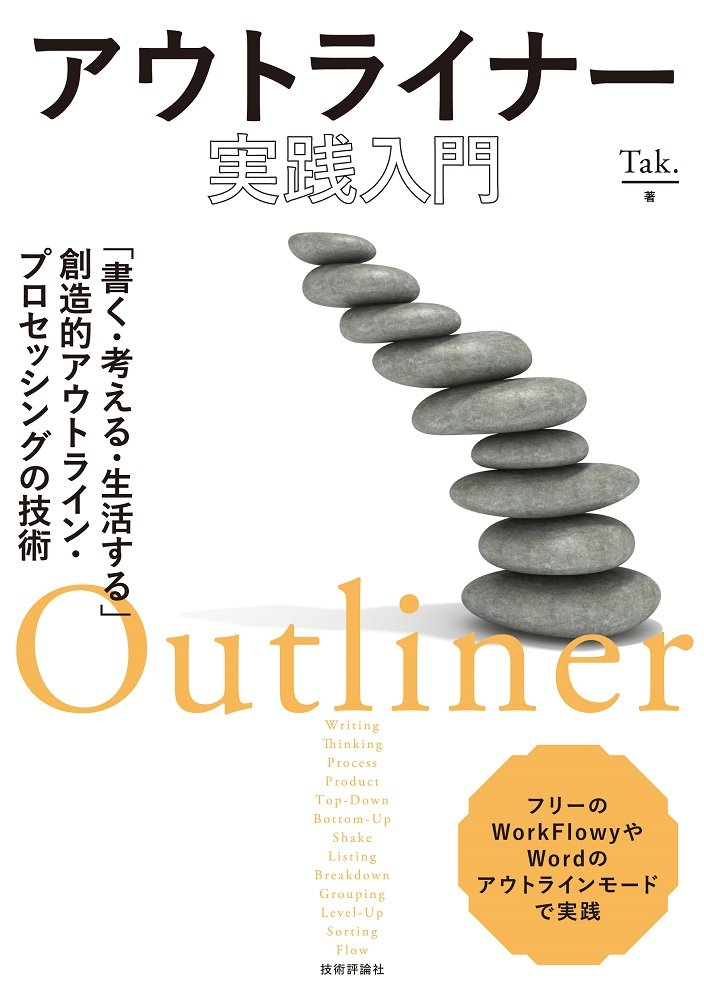
\includegraphics[height=3cm]{images/4774182850}
        \caption{アウトライナー実践入門 ~「書く・考える・生活する」創造的アウトライン・プロセッシングの技術~\cite{2016tak_book}}
        \label{fig:tak_book}
    \end{minipage}
\end{figure}

\chapter{まとめ}


\bibliographystyle{csg-thesis}
\bibliography{ {{ .Id }}}  %% thesis.bib というファイルを用意

% 付録が必要ならつける
\appendix
\chapter{プログラム例}


\end{document}
